The SM background can be catogrized into the irreducible and reducible background.
The irreducible background includes events containing two prompt leptons, \met, and jets.
The reducible background includes events containing fake/non-prompt leptons.
Since the background estimations rely on the choice of the control regions (CRs) and validation regions (VRs) heavily, the concepts of the CRs and VRs are introduced in Sect.~\ref{sec:bkg_control_and_validation_regions}.
The detail discussions of the irreducible background is presented in Sect.~\ref{sec:bkg_irreducible_background} and of the reducible background is described in Sect.~\ref{sec:bkg_reducible_background}.
Finally, the systematic uncertainty study for this analysis is mentioned in Sect.~\ref{sec:bkg_systematic_uncertainties}.

%%%
%%%
%%%

\section{Control and validation regions}
\label{sec:bkg_control_and_validation_regions}

%%%
%%%
%%%

\subsection{The concepts}
\label{subsec:bkg_SRs_CRs_VRs_concepts}
Three different data regions are considered in any physics analysis: signal region (SR), control region (CR), and validation region (VR).
The SR is a signal-enriched region, the CR is a background-enriched region, and the VR is a region used to validate the robustness of the signal and background predictions.
The SR is a particular region of phase space where a set of selection criteria are applied on kinematic observables.
In the SR, the number of predicted signal events have a significant excess over the number of predicted background events.
The CR is enriched in a particular background process with low expected contamination from the signals considered, designed to be similiar to SR in the kinematic properties, and kept statistically independent from the SR.
The background contamination in the SR can be estimated by extrapolating from the CR.
The VR, usually placed in between the SR and CR, is used to validate the predicted number of background events in the SR.
Figure~\ref{fig:bkg_SRs_CRs_VRs} shows the concepts of multiple SRs, CRs, and VRs.

\begin{figure}[htbp]
    \begin{center}
        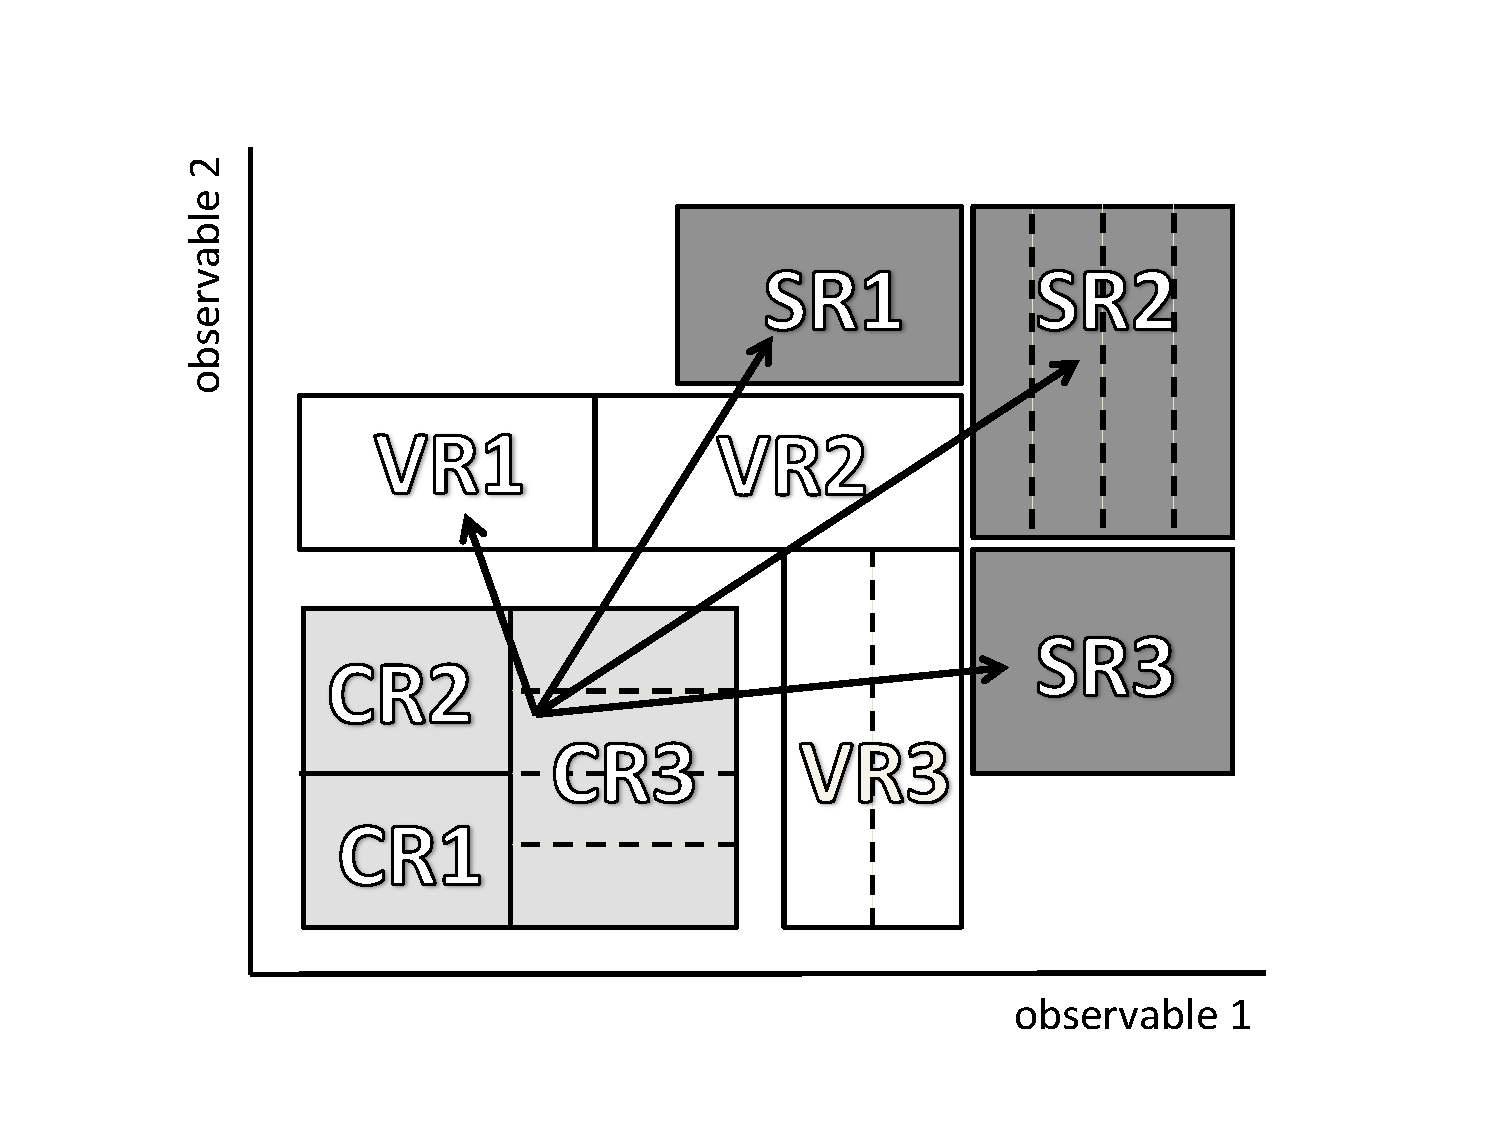
\includegraphics[scale=0.5]{cartoon_CRVRSR_bw.pdf}
        \caption{A illustration of multiple signal, control, and validation regions.
        The background contamination in the SRs can be estimated by extrapolating from the CRs and is verified in the VRs which lie in between the SRs and CRs.
        All regions can be single bin or multiple bins which are indicated by the dashed lines.
        The figure is taken from~\cite{Baak:2014wma}.}
        \label{fig:bkg_SRs_CRs_VRs}
    \end{center}
\end{figure}

%%%
%%%
%%%

\subsection{Specific to this analysis}
\label{subsec:bkg_SRs_CRs_VRs_spicific}
Table~\ref{tab:bkg_background_processes} lists the SM background processes for this analysis, the origins in the SR, and the estimation strategies.
In order to estimate and validate the background contaminations in SR, two CRs and three VRs are defined.
Table~\ref{tab:bkg_CRs_VRs_definitions} lists the definitions of CRs and VRs where the common selection criteria listed in Table~\ref{tab:event_signal_region} have been applied.
The CR-top is used to estimate the \ttbar and $tW$ contaminations in SR.
The CR-tau is used to estimate the  $Z^{(*)}/\gamma^{*}(\to \tau \tau)$+jets contamination in SR.
The VR-VV is used for validating diboson background, the VR-SS is used for validating same-sign dilepton background, and VRDF-$m_{\ell \ell}$ is used for validating the background come from different flavor leptons, which include both $e \mu$ and $\mu e$.

\begin{table}[htbp]
    %\begin{center}
    \resizebox{\textwidth}{!}{% <------ Don't forget this %
        \begin{tabular}{lll}
            \hline
            \hline
            Background process                             & Origin in SR                                             & Estimation strategy\\
            \hline
            \ttbar, $tW$ ($\to 2\ell$)                     & irreducible, $b$-jet fails identification                & CR using $b$-tagging\\
            $Z^{(*)}/\gamma^{*}(\to \tau \tau)$+jets       & irreducible fully leptonic $\tau$                        & CR using $m_{\tau \tau}$\\
            $Z^{(*)}/\gamma^{*}(\to ee, \mu \mu)$+jets     & instrumental \met                                        & MC\\
            loss mass Drell-Yen                            & instrumental \met                                        & MC, data-driven cross check\\
            fakes ($W$+jets, $VV(1\ell)$, \ttbar($1\ell$)) & jet fakes $2^\mathrm{nd}$ lepton                         & fake factor, SS VR\\
            $VV$                                           & irreducible dileptonic and missed $3^\mathrm{rd}$ lepton & MC, VR using $\met/H_\mathrm{T}^\mathrm{leptons}$\\
            orther rare processes                          & irreducible leptonic decays                              & MC\\
            \hline
            \hline
        \end{tabular}
    }
    %\end{center}
    \caption{The background processes for the 2$\ell$ analysis and the strategy for estimating the background contamination in the SR.}
    \label{tab:bkg_background_processes}
\end{table}

\begin{table}[htbp]
    %\begin{center}
    \resizebox{\textwidth}{!}{% <------ Don't forget this %
        %{\scriptsize
            \begin{tabular}{llll}
                \hline
                \hline
                Region               & Leptons                                                                        & $\met/H_{\mathrm{T}}^{\mathrm{lep}}$                & Additional requirements\\
                \hline
                CR-top               & $e^{\pm}e^{\mp}$, $\mu^{\pm}\mu^{\mp}$, $e^{\pm}\mu^{\mp}$, $\mu^{\pm}e^{\mp}$ & $> 5$                                               & $\ge 1 b$-tagged jet(s)\\
                CR-tau               & $e^{\pm}e^{\mp}$, $\mu^{\pm}\mu^{\mp}$, $e^{\pm}\mu^{\mp}$, $\mu^{\pm}e^{\mp}$ & $\in$ [4, 8]                                        & $m_{\tau \tau} \in$ [60, 120]~{\GeV}\\
                \hline
                VR-VV                & $e^{\pm}e^{\mp}$, $\mu^{\pm}\mu^{\mp}$, $e^{\pm}\mu^{\mp}$, $\mu^{\pm}e^{\mp}$ & $< 3$                                               & -\\
                VR-SS                & $e^{\pm}e^{\pm}$, $\mu^{\pm}\mu^{\pm}$, $e^{\pm}\mu^{\pm}$, $\mu^{\pm}e^{\pm}$ & $> 5$                                               & -\\
                VRDF-$m_{\ell \ell}$ & $e^{\pm}\mu^{\mp}$, $\mu^{\pm}e^{\mp}$                                         & $>$ max(5, 15 - 2 $m_{\ell \ell}/1~{\GeV}$)         & $\Delta R_{\ell \ell} < 2$, $m_{\mathrm{T}}^{\ell_{1}} < 70$~{\GeV}\\
                \hline
                \hline
            \end{tabular}
        %}
    }
    %\end{center}
    \caption{Definition of control regions and validation regions.}
    \label{tab:bkg_CRs_VRs_definitions}
\end{table}%

%%%
%%%
%%%

\section{Irreducible background}
\label{sec:bkg_irreducible_background}
The irreducible background for this analysis are the SM processes containing two prompt leptons, \met, and jets.
Therefor, they can enter the SR and mimic the signal events.
The dominant sources are the \ttbar, $tW$, and $Z^{(*)}/\gamma^{*}(\to \tau \tau)$+jets processes.
These processes decay to same flavor lepton pairs ($ee$ and $\mu \mu$) and different flavor lepton pairs ($e \mu$ and $\mu e$) at the same rates.
When defining the CR-top and CR-tau, all possible flavor $e^{\pm} e^{\mp}$, $\mu^{\pm} \mu^{\mp}$, $e^{\pm} \mu^{\pm}$, $\mu^{\pm} e^{\mp}$ are consider to enhance the statistics.
By requiring the events with at least one $b$-tagged jet, the CR-top defined a top quarks enriched region with $\sim$72\% purity.
The CR-top is used to estimate the \ttbar and $tW$ decaying to 2$\ell$ final states in the SR.
By requiring the events satisfying $60 < m_{\tau \tau} < 120$~{\GeV} and $\met/H_{\mathrm{T}}^{\mathrm{lep}}$ between 4 and 8 to reduce the signal contaminations, the CR-tau defined a $Z^{(*)}/\gamma^{*}(\to \tau \tau)$+jets enriched region with $\sim$80\% purity.
The CR-tau is used to estimate the leptonic $\tau$ contaminations in the SR.
The kinematic distributions of $\met/H_\mathrm{T}^\mathrm{lep}$ and $m_{\tau \tau}$ in the CR-top and CR-tau after performing background-only fit are shown in Fig~\ref{fig:bkg_kinematic_distributions_in_CRs}.
All the event selection criteria are applied except the variable being plotted.
The expected background contributions from different processes are stacked and compared with the data.

\begin{figure}[ht]
    \begin{center}
        \begin{subfigure}[b]{0.48\textwidth}
            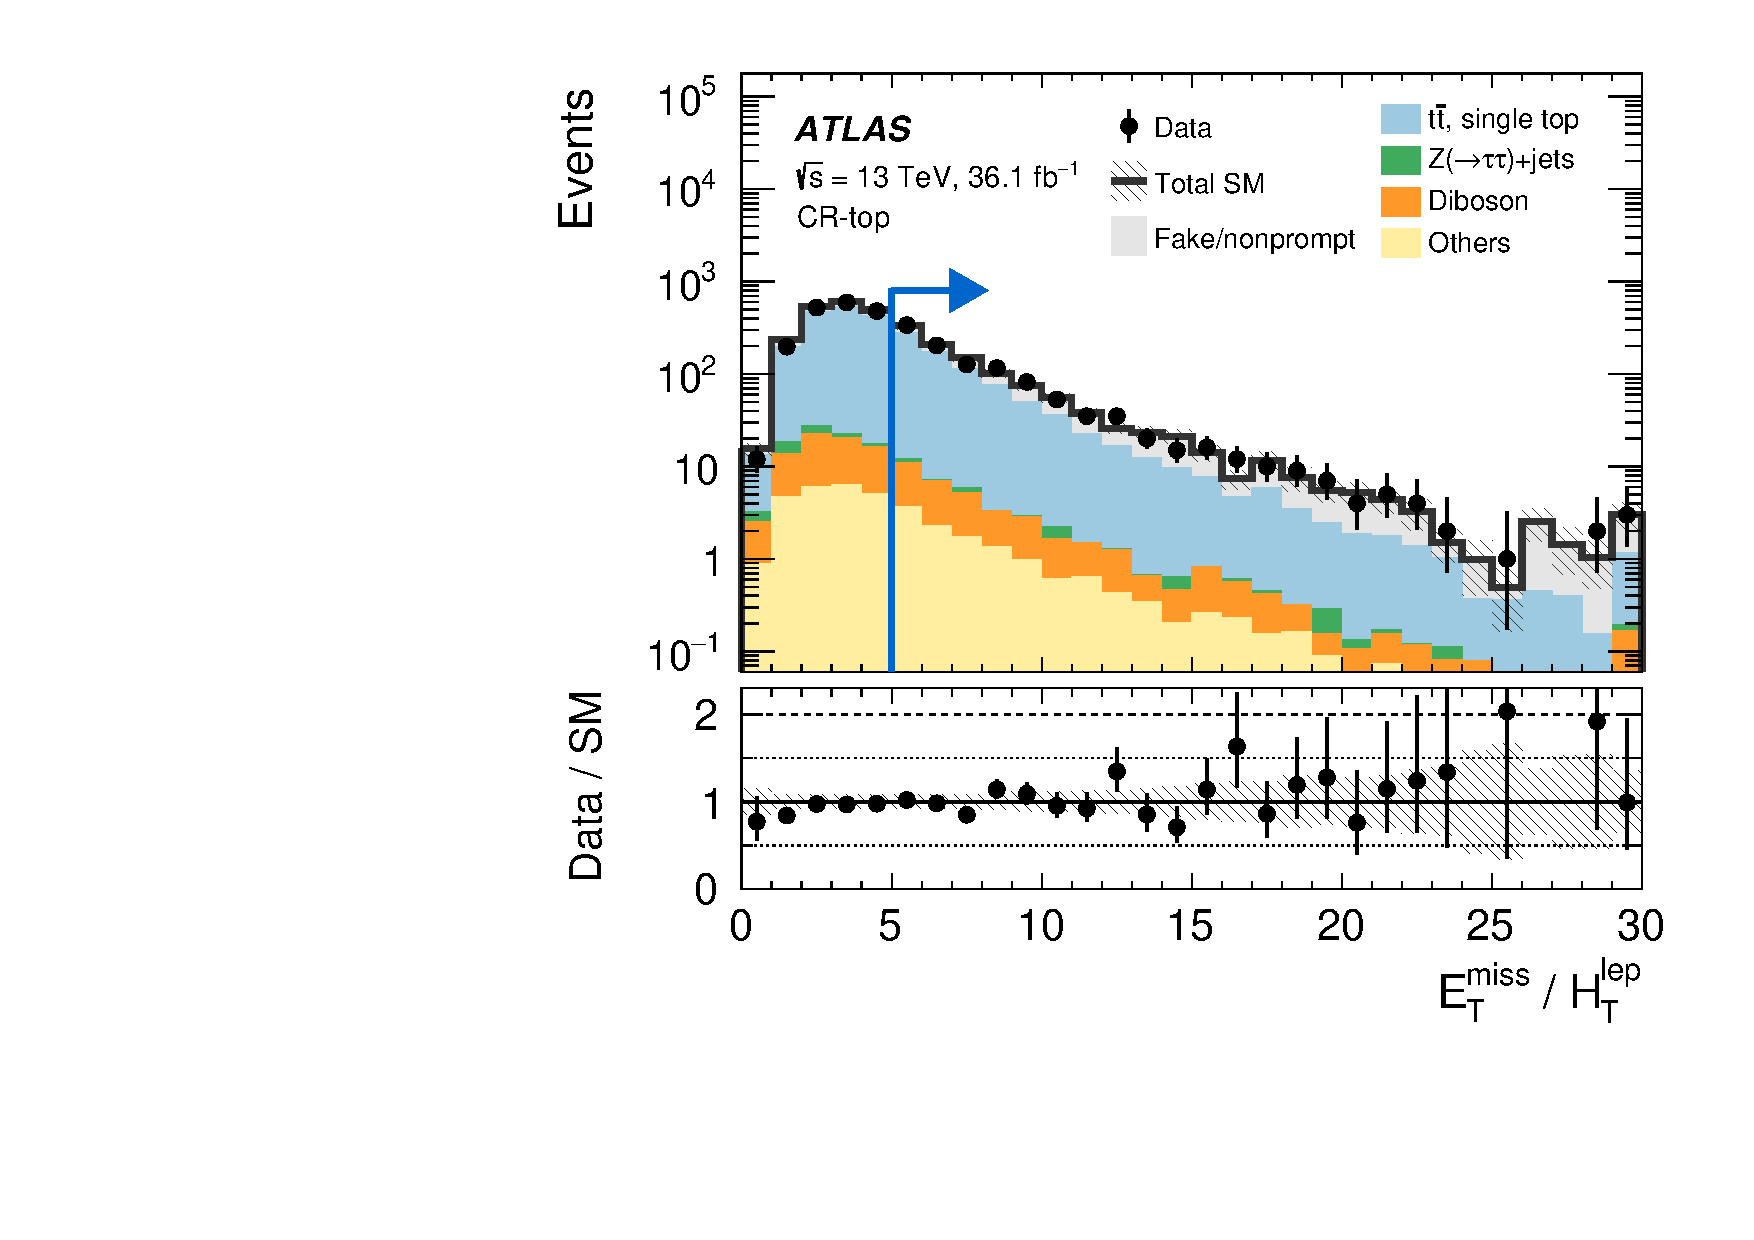
\includegraphics[scale=0.4]{Higgsino_bkg_CRtop_CRtop_METOverHTLep_METOverHTLep.pdf}
            \caption{The $\met/H_\mathrm{T}^\mathrm{lep}$ distribution in CR-top.}
            \label{}
        \end{subfigure}
        \begin{subfigure}[b]{0.48\textwidth}
            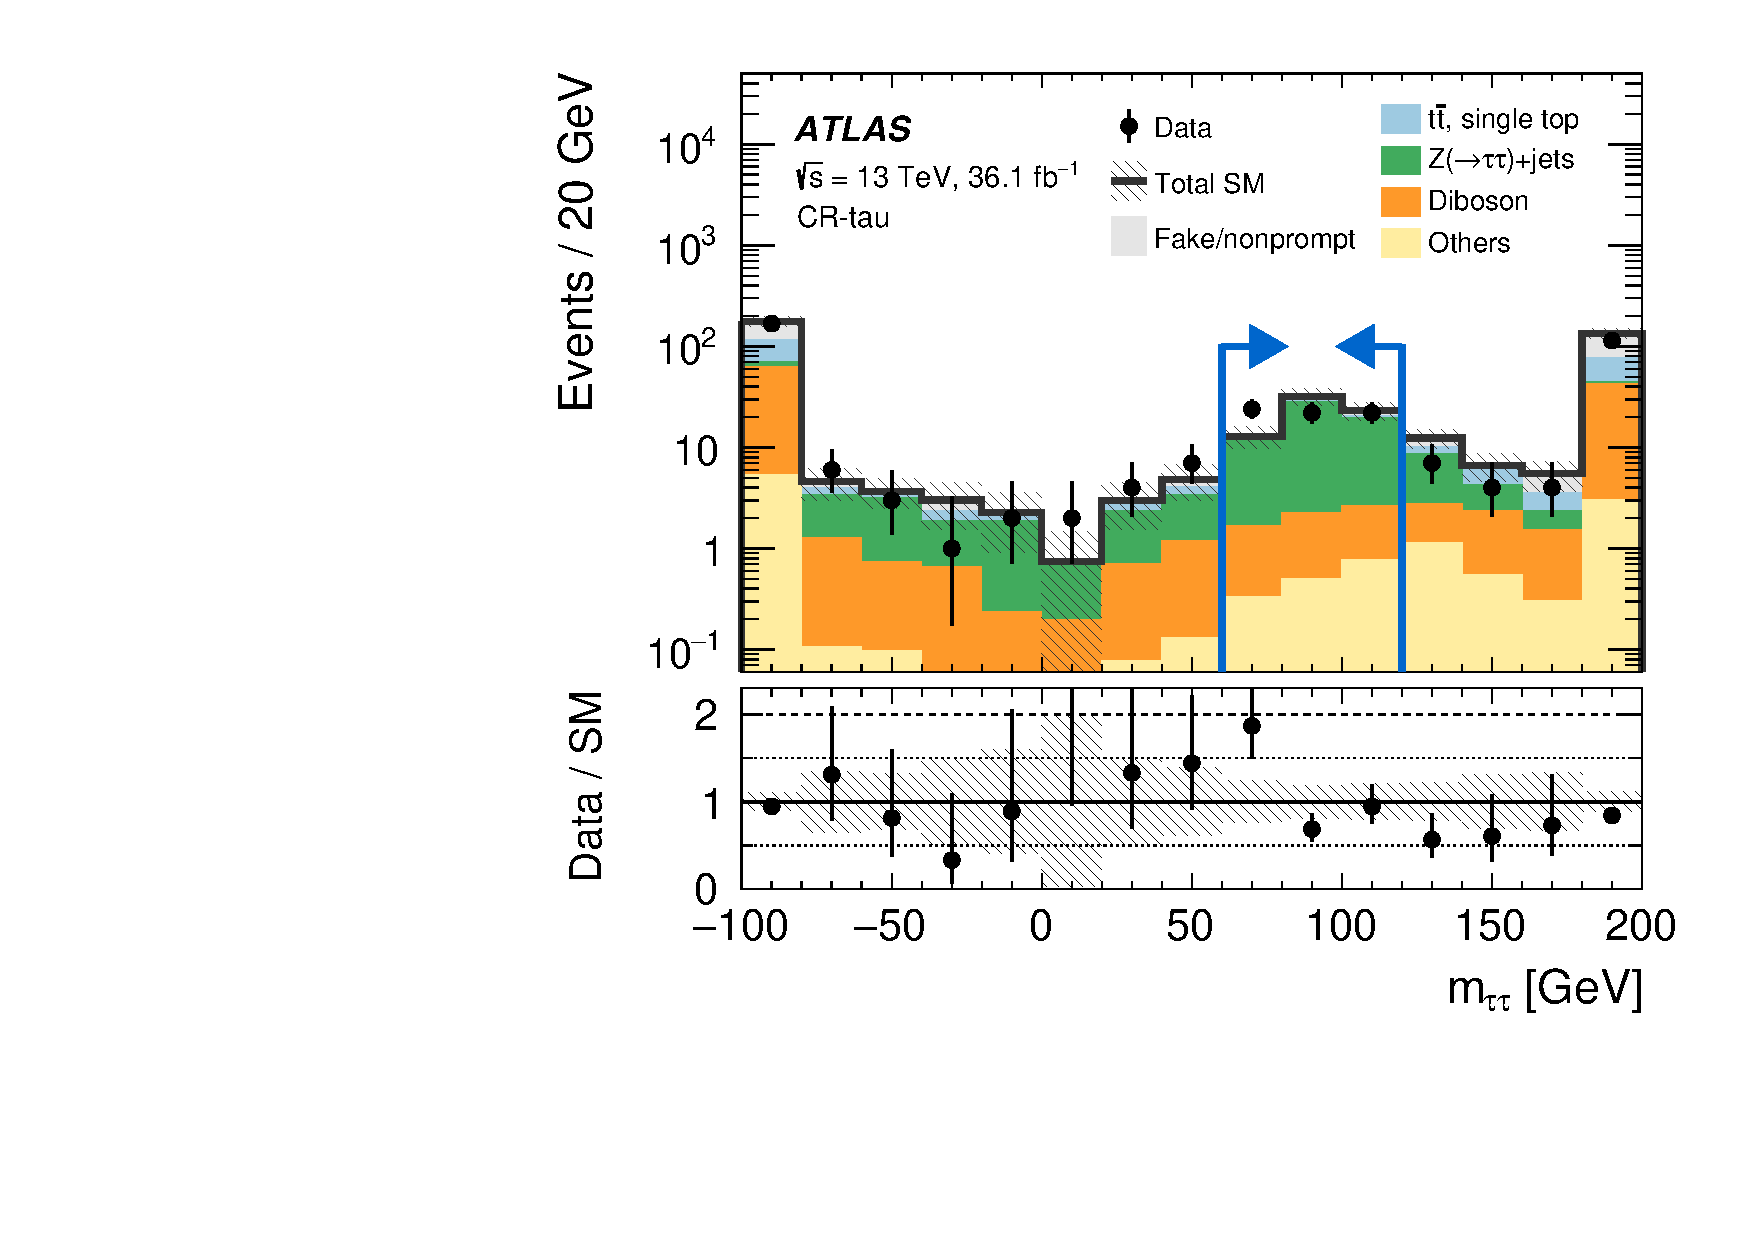
\includegraphics[scale=0.4]{Higgsino_bkg_CRtau_CRtau_MTauTau_MTauTau.pdf}
            \caption{The $m_{\tau \tau}$ distribution in CR-tau.}
            \label{}
        \end{subfigure}
        \caption{The kinematic distributions of $\met/H_\mathrm{T}^\mathrm{lep}$ and $m_{\tau \tau}$ in the CR-top and CR-tau, respectively.
        All the event selection criteria are applied except the variable being plotted and the bickground-only fits are performed.
        The selection requirement of the plotting variable is indicated by the blue arrows.
        The first and last bins include the underflow and overflow, respectivley.
        The expected background contributions from different processes are stacked and compared with the data.}
        \label{fig:bkg_kinematic_distributions_in_CRs}
    \end{center}
\end{figure}

The diboson $VV$ events and the rare processes are also contributioned to the irreducible background.
But it is difficult to have pure diboson or rare sample that can be used to estimate the contaminations in SR.
Therefore, the background contaminations are estimated using MC simulation and validated by the VR-VV.
By requiring $\met/H_\mathrm{T}^\mathrm{lep} < 3$, the signal contamination in the VR-VV is at most 8\% in the samples, the diboson events contribute $\sim$40\%, fake lepton events contribute $\sim$25\%, \ttbar and single top events contribute $\sim$23\%, and the rest parts are smaller and contributed by the other processes.

The VRDF-$m_{\ell \ell}$ validation region is construced using different flavor ($e\mu$ and $\mu e$) leptons.
This VR has the same selection criteria as the SR, except the leptons are composed by different flavor.
Since the irreducible background are symmetric in $ee+\mu\mu$ and $e\mu+\mu e$, the VRDF-$m_{\ell \ell}$ is used to check the eventual extrapolation in the fitting procedure within the same kinematic as SR.
The signal contamination in this VR is less than 8\%.

%%%
%%%
%%%

\section{Reducible background}
\label{sec:bkg_reducible_background}
The main contributions of the reducible background come from the non-prompt leptons and the processes that the reconstructed \met are instrumental in origin.

%%%
%%%
%%%

\subsection{Fake/non-prompt lepton background}
\label{subsec:bkg_fake_lepton_background}
The background of non-prompt leptons, or called fake leptons, mainly come from the $W$+jets, VV, \ttbar processes.
In these processes, a jet is misidentified as a lepton and form a dilepton final state in the SR.
Because the MC simulation couldn't model fake leptons well, a data-driven Fake Factor method~\cite{ATLAS:2014aga} is used to estimate the fake lepton contamination in the SR. 

%%%
%%%
%%%

\subsubsection{Faje factor method}
\label{subsubsec:bkg_fake_factor_method}
The Fake Factor method defined a tight set and a loose set of lepton identification ceiteria.
The tight set refers as ID and the loose set refers as anti-ID.
The ID criteria correspond to the requirements applied to signal leptons used in the analysis.
The anti-ID criteria define a sample enriched in fake leptons by releasing or inverting one or more of the identification, isolation, or $|d_{0}|/\sigma(d_{0})$ requirements relative to the signal leptons.
There the lepton samples in ID and anti-ID are orthogonal.
Then the fake factor $F$ is defined as the ratio between the number of ID and the number of anti-ID leptons as shown in Eq.~\ref{eq:bkg_fake_factor}.

\begin{equation}
    F = \frac{N_\mathrm{ID}}{N_\mathrm{anti-ID}}
    \label{eq:bkg_fake_factor}
\end{equation}

The $F$ for electron and muon are measured in a fake leptons enriched region as a function of reconstructed lepton \pt and are used to estimate the reducible background in the SR.
These $F$ are applied to events in a measurement region which has the same selection criteria as SR, except an ID lepton is replaced by an anti-ID lepton.






%%%
%%%
%%%

\subsection{Instrumental \met background}
\label{subsec:bkg_instrumental_met_background}
Because the detector mismeasuring leptons or jets in the background processes cause the high offline \met in SR, the contributions arise from these background processes, for example, Drell-Yan dilepton production are studied using MC samples.
By requiring $\met > 200$~{\GeV}, the contributions from these background processes are expected very small.
By vetoing $J/\psi$ peak, $3.0 < m_{\ell \ell} < 3.2$~{\GeV}, the contributions from $J/\psi$ resonance can be removed efficiently.
By requiring min($\Delta \phi($any jet, $\mathbf{p}^{\mathrm{miss}}_{\mathrm{T}})) > 0.4$, the events contain mismeasured jet causing large \met can be suppressed.
After applying these requirements, the instrumental \met background are foound to be negligible.

%%%
%%%
%%%

\section{Systematic uncertainties}
\label{sec:bkg_systematic_uncertainties}

%%%
%%%
%%%

%\begin{table}[ht]
%    \begin{center}
%        {\scriptsize
%            \begin{tabular}{llll}
%                \hline
%                \hline
%                Region               & Leptons                                                                        & $\met/H_{\mathrm{T}}^{\mathrm{lep}}$                & Additional requirements\\
%                \hline
%                CR-top               & $e^{\pm}e^{\mp}$, $\mu^{\pm}\mu^{\mp}$, $e^{\pm}\mu^{\mp}$, $\mu^{\pm}e^{\mp}$ & $> 5$                                               & $\ge 1 b$-tagged jet(s)\\
%                CR-tau               & $e^{\pm}e^{\mp}$, $\mu^{\pm}\mu^{\mp}$, $e^{\pm}\mu^{\mp}$, $\mu^{\pm}e^{\mp}$ & $\in$ [4, 8]                                        & $m_{\tau \tau} \in$ [60, 120]~{\GeV}\\
%                \hline
%                VR-VV                & $e^{\pm}e^{\mp}$, $\mu^{\pm}\mu^{\mp}$, $e^{\pm}\mu^{\mp}$, $\mu^{\pm}e^{\mp}$ & $< 3$                                               &\\
%                VR-SS                & $e^{\pm}e^{\mp}$, $\mu^{\pm}\mu^{\mp}$, $e^{\pm}\mu^{\mp}$, $\mu^{\pm}e^{\mp}$ & $> 5$                                               &\\
%                VRDF-$m_{\ell \ell}$ & $e^{\pm}\mu^{\mp}$, $\mu^{\pm}e^{\mp}$                                         & $>$ max(5, 15 - 2 $\frac{m_{\ell \ell}}{1~{\GeV}}$) & $\Delta R_{\ell \ell} < 2$, $m_{\mathrm{%T}}^{\ell_{1}} < 70$~{\GeV}\\
%                \hline
%                \hline
%            \end{tabular}
%        }
%    \end{center}
%    \caption{Definition of control regions and validation regions.}
%    \label{tab:bkg_}
%\end{table}%
